%! Author = anton
%! Date = 31/08/2024

\subsection{Calibration Consideration On Selected Models}
\label{subsec:bestModels}
\textbf{Best Models}

For each method, the best configuration was chosen by looking at the minDCF parameter, so the best configurations are:

\begin{itemize}
    \item \textbf{Logistic Regression}: \(\lambda=3.162*10^{-2}\), minDCF is 0.2436 and actDCF is 0.4972
    \item \textbf{Support Vector Machine}: with RBF Kernel with \(\gamma=0.1\) and \(C=100\), minDCF is 0.1845 and actDCF is 0.3581
    \item \textbf{Gaussian Mixture Model}: with Diagonal convolution and \((nc0=8, nc1=32)\) where \(nc0\) is the number of
    component for class 0 and \(nc1\) is number of component for class 1, minDCF is 0.1312 and actDCF is 0.1517
\end{itemize}

In \autoref{fig:BestConfiguration} we see the behaviour of the 3 best models we have selected, now we will apply the calibration to these.

\begin{figure}[h!]
    \centering
    \begin{subfigure}[b]{0.30\linewidth}
        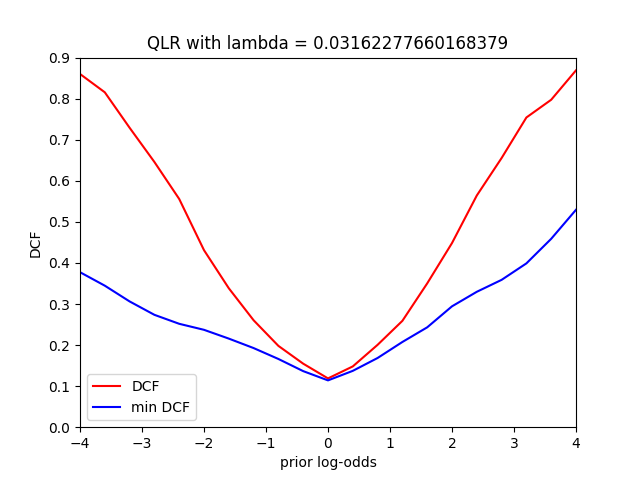
\includegraphics[width=\linewidth]{Lab/11. Lab 11/Images/BestConfiguration/01. QLR}
        \label{fig:QLRBest}
    \end{subfigure}
    \begin{subfigure}[b]{0.30\linewidth}
        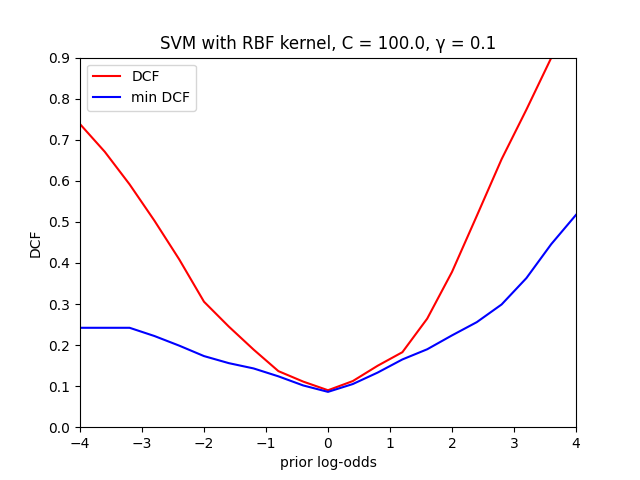
\includegraphics[width=\linewidth]{Lab/11. Lab 11/Images/BestConfiguration/02. SVM}
        \label{fig:SVM}
    \end{subfigure}
    \begin{subfigure}[b]{0.30\linewidth}
        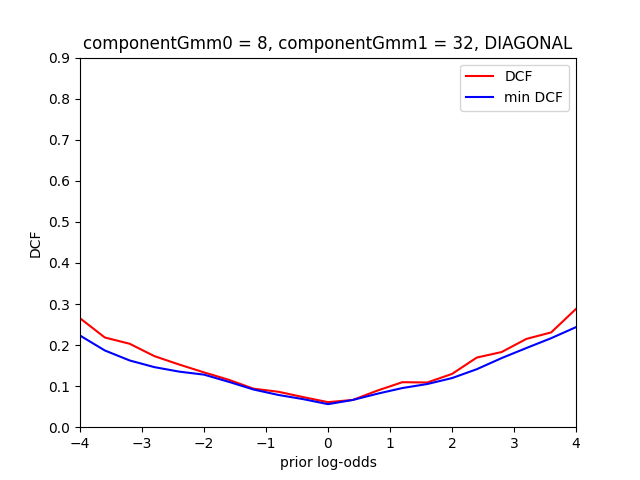
\includegraphics[width=\linewidth]{Lab/11. Lab 11/Images/BestConfiguration/03. GMM}
        \label{fig:GMM}
    \end{subfigure}
    \caption{Shows minDCF and actDCF for three best models}
    \label{fig:BestConfiguration}
\end{figure}

\subsection{Calibration Scores For Best Models}
\label{subsec:calibrationScores}
The evaluation is based on the theoretical threshold:
\begin{equation}
    t= - \log \frac{\tilde{\pi}}{1 - \tilde{\pi}}
    \label{eq:threshold}
\end{equation}

The threshold expressed in the \autoref{eq:threshold} does not guarantee that it is the optimal one,
so a score analysis is applied.
The function \(f\) that maps the uncalibrated score to the calibrated score has the form:

\begin{equation}
    f(s) = \alpha s + \beta
    \label{eq:eqCalibration}
\end{equation}

\autoref{eq:logLikelihoodCalibration} can be interpreted as log-likelihood of the two classes:

\begin{equation}
    f(s) = \log {\frac{f_{S\mid C}(s\mid H_T)} {f_{S\mid C}(s\mid H_F)}} = \alpha s + \gamma
    \label{eq:logLikelihoodCalibration}
\end{equation}

Instead, class posterior probability for prior \(\tilde{\pi}\) is:

\begin{equation}
    \log {\frac{P(C=H_T\mid s)}{P(C=H_F\mid s)}} = \alpha s + \gamma + \log \frac{\tilde{\pi}}{1 - \tilde{\pi}}
    \label{eq:posteriorProbability}
\end{equation}

From the previous equations we can write that:
\begin{equation}
    \beta = \gamma + \log \frac{\tilde{\pi}}{1 - \tilde{\pi}}
    \label{eq:beta}
\end{equation}

\autoref{eq:logLikelihoodCalibration} can be rewritten as:
\begin{equation}
    f(s) = \alpha s + \gamma = \alpha s + \beta - \log \frac{\tilde{\pi}}{1 - \tilde{\pi}}
    \label{eq:logLikelihoodCalibrationBeta}
\end{equation}

\subsection{Result Calibration}
\label{subsec:resultCalibration}
We apply calibration to the models we have chosen, so as to improve the actual performance by making them more similar
to the predicted performance.
Basically, we try to reduce the gap between minDCF and actDCF .
In the \autoref{tab:resultUnCalibratedAndCalibratedModels} shows the results of the different models after calibration;
the calibration was applied using different \(\tilde{\pi}\) as shown in the table.
The best results are obtained by applying GMM with a prior of 0.1 0.5

\begin{figure}[h!]
    \centering
    \begin{subfigure}[b]{0.40\linewidth}
        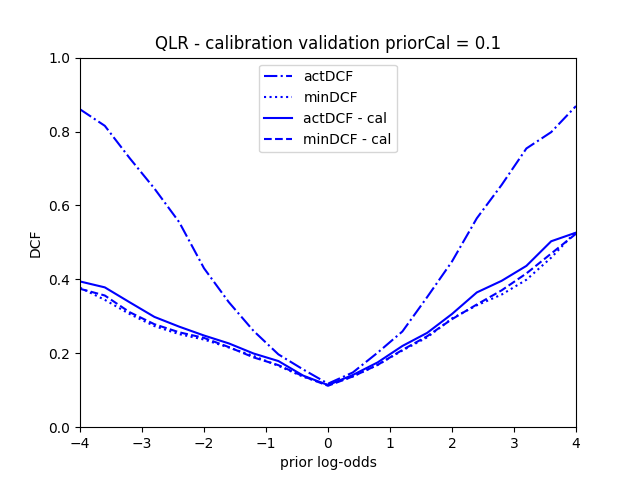
\includegraphics[width=\linewidth]{Lab/11. Lab 11/Images/CalibrationAndFusion/01. QLR}
        \label{fig:QLRCalibration}
    \end{subfigure}
    \begin{subfigure}[b]{0.40\linewidth}
        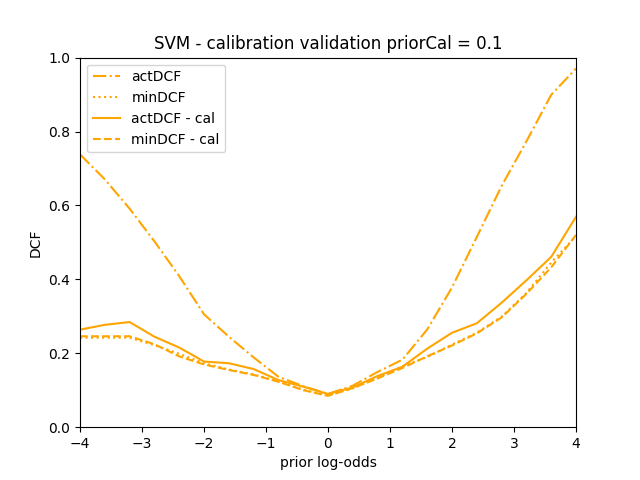
\includegraphics[width=\linewidth]{Lab/11. Lab 11/Images/CalibrationAndFusion/02. SVM}
        \label{fig:SVMCalibration}
    \end{subfigure}
    \begin{subfigure}[b]{0.40\linewidth}
        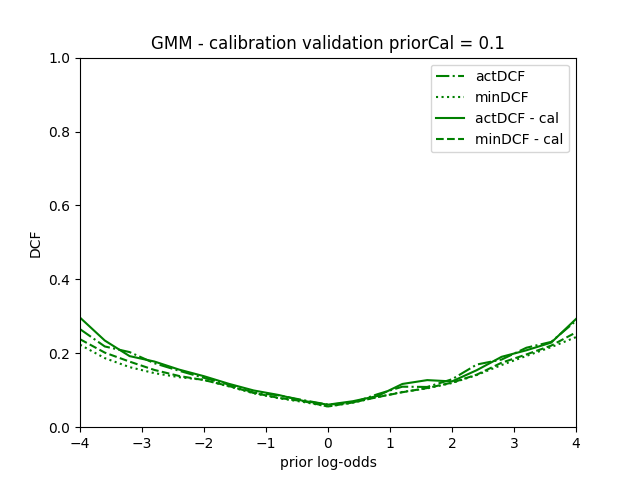
\includegraphics[width=\linewidth]{Lab/11. Lab 11/Images/CalibrationAndFusion/03. GMM}
        \label{fig:GMMCalibration}
    \end{subfigure}
    \begin{subfigure}[b]{0.40\linewidth}
        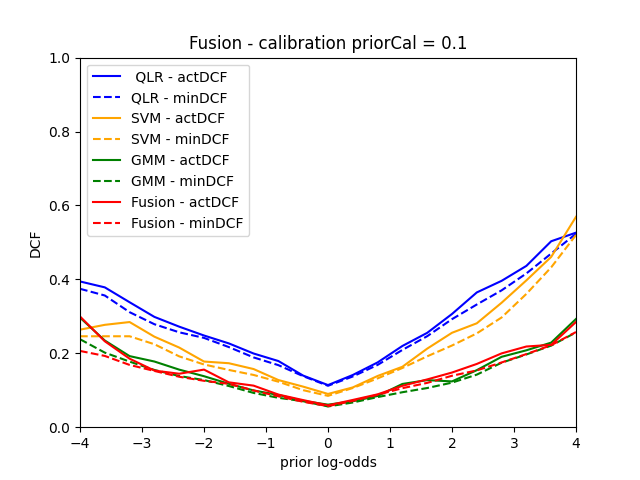
\includegraphics[width=\linewidth]{Lab/11. Lab 11/Images/CalibrationAndFusion/04. Fusion}
        \label{fig:FusionCalibration}
    \end{subfigure}
    \caption{Shows result of each model before and after calibration}
    \label{fig:BestConfigurationCalibration}
\end{figure}


\begin{table}[h!]
    \centering
    \begin{tabular}{>{\centering\arraybackslash}p{2.9cm} >{\centering\arraybackslash}p{2.9cm} >{\centering\arraybackslash}p{2.9cm} >{\centering\arraybackslash}p{2.9cm}}
        \toprule
        & \multicolumn{3}{c}{\textbf{Uncalibrated Models [minDCF - actDCF]}} \\
        \midrule
        \textbf{QLR} & \multicolumn{3}{c}{0.2436 - 0.4972} \\
        \textbf{SVM} & \multicolumn{3}{c}{0.1845 - 0.3581} \\
        \textbf{GMM} & \multicolumn{3}{c}{0.1312 - 0.1517} \\
        \midrule
        \midrule
        & \multicolumn{3}{c}{\textbf{Calibrated Models [minDCF - actDCF]}} \\
        \midrule
        & \(\tilde{\pi} = 0.1\) & \(\tilde{\pi} = 0.5\) & \(\tilde{\pi} = 0.9\) \\
        \midrule
        \textbf{QLR}    & 0.2486 - 0.2721       & 0.2496 - 0.2609       & 0.2480 - 0.2657       \\
        \textbf{SVM}    & 0.1794 - 0.1894       & 0.1814 - 0.2032       & 0.1881 - 0.2020       \\
        \textbf{GMM}    & 0.1324 - 0.1518       & 0.1314 - 0.1518       & 0.1283 - 0.1559       \\
        \midrule
        \textbf{Fusion} & 0.1304 - 0.1568       & 0.1373 - 0.1639       & 0.1382 - 0.1731       \\
        \bottomrule
    \end{tabular}
    \captionsetup{justification=justified,singlelinecheck=false,format=hang}
    \caption{Show minDCF and actDCF for different models before and after calibration}
    \label{tab:resultUnCalibratedAndCalibratedModels}
\end{table}

\autoref{fig:BestConfigurationCalibration} shows the Bayes error graphs of the different methods with a calibration prior of 0.1.
We can see that an improvement can be observed for all configurations after calibration.
Instead, by applying fusion, the scores of the different models are combined in an attempt to have an overall improvement,
but it can be observed that the values of this method are very similar to those of GMM and are also less calibrated.

\newpage
\textbf{Summarize}\par
Looking at the various outcomes, it is determined that the best method is GMM by applying a diagonal covariance matrix, as it is the one with the best minDCF and actDCF values.
